\subsection{Why is a website important?}

A website is the most efficient way to represent the product as well as the project team. In case of OctoTagger the website also fulfils the task to distribute the product by offering a download. As web developer it's necessary to keep the target audience in mind and adjust the website to its needs.

\subsection{Concept of OctoTagger website}

The website of OctoTagger follows simple and decent design guidelines. It was designed to satisfy the users needs and being as lightweight as possible at the same time. Only few and small images are used on the entire site keeping loading times short.

A major aspect of the website is the ultra-lightweight, straight and modern design. The image design was kept clear and simple without the use of explicit borders. Due to that images appear flat and homogeneous.

\subsubsection{Usability}

The site was developed to be intuitive and easy to use. The user can reach every page independent of his current position.

To make navigation easier, clickable items were made as distinctive as possible. Only buttons and elements of the navigation bar respond to mouse clicks. These objects are also the only ones to respond to hovering, so the user gets signalled that after a click an action will be performed.

As an example for usability, downloading Octotagger could hardly be easier. Every button leading to a download, is colored in a shade of green, compared to other buttons colored in a shade of blue. In fact the user just has to click every green button, follow some installation instructions and is able to use Octotagger after a few minutes.

\subsubsection{Responsive Design}

The challenge for web development is to create a website, that looks good on every available screen size and device like desktop PCs, tablets, phablets and mobile phones. This can be ensured through different solutions.

The first option is to write different CSS sheets for every screen size or device, which requires the most work.

An easier possibility is called responsive design and there are numerous frameworks to support the developer with it. 

Responsive design means that a website is created to work on every device and adapts its appearance based on the screen size and orientation. The concept is based on flexible grids and layouts and the use of CSS media queries.

The following images show the OctoTagger website adapted to different screen sizes.

\begin{center}
\begin{tabular}{ c  c c }
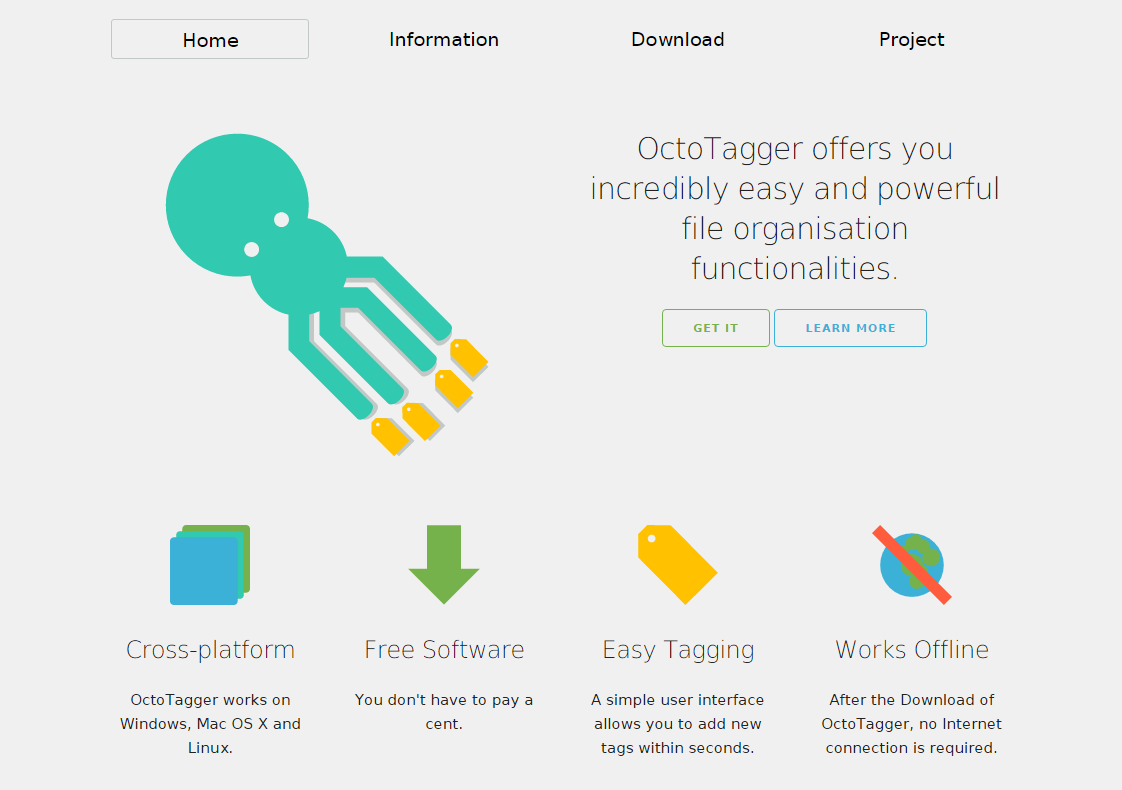
\includegraphics[scale=0.20]{images/home_full.png} & 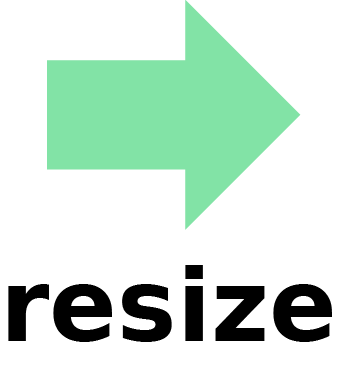
\includegraphics[scale=0.30]{images/resize.png} & 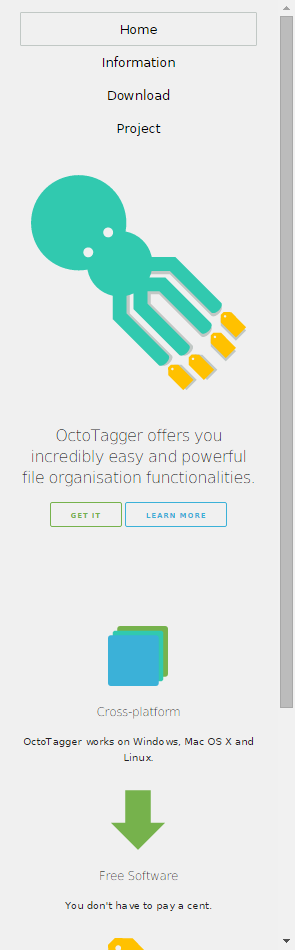
\includegraphics[scale=0.30]{images/home_small.png} \\
\end{tabular}
\end{center}

When the website passes a threshold during the resize, so that the elements are positioned above each other to fit the smaller screen width. The framework (see \ref{sec:Skeleton}) stacked the elements automatically, but adjustments were still necessary. Some media queries (see \ref{sec:MediaQueries}) had to be adapted so that elements fit perfectly together.

\paragraph{Flexible Grid} \hspace{0pt} \\

Most responsive framework rely on a flexible grid system, with typically 12 columns. Elements in the HTML code can now be positioned within this grid with the help of CSS classes. Depending on the width you want a HTML object to have, you have to give the proper CSS classes.

The image below shows a flexible grid example using the Skeleton framework (see \ref{sec:Skeleton})

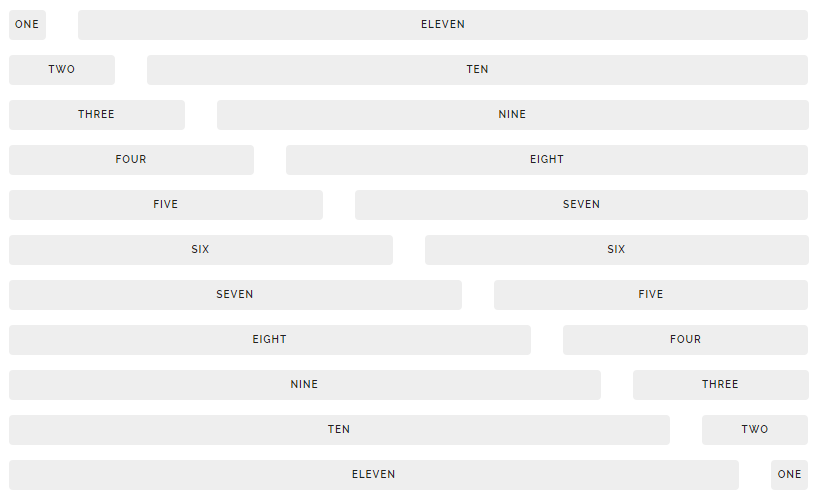
\includegraphics[scale=0.50]{images/skeleton_grid.png} 

\paragraph{CSS Media Queries} \hspace{0pt} \\
\label{sec:MediaQueries}

With the help of CSS Media Queries it's possible to set CSS attributes depending on conditions like screen width and device type. For instance the width of a box can  be increased when the window is enlarged.

The following code snippet shows an example for some width dependant media queries.

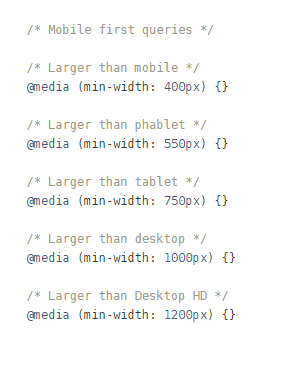
\includegraphics[scale=0.70]{images/media_query.png} 




\subsubsection{Corporate Design}

\subsection{Structure}

The OctoTagger website is basically made up of four pages called Home, Information, Download and Project. All these pages are accessible via the navigation bar which is positioned on the top on every page. In addition there are several sub-pages only accessible on the download site.

\subsubsection{Home page}

\begin{center}
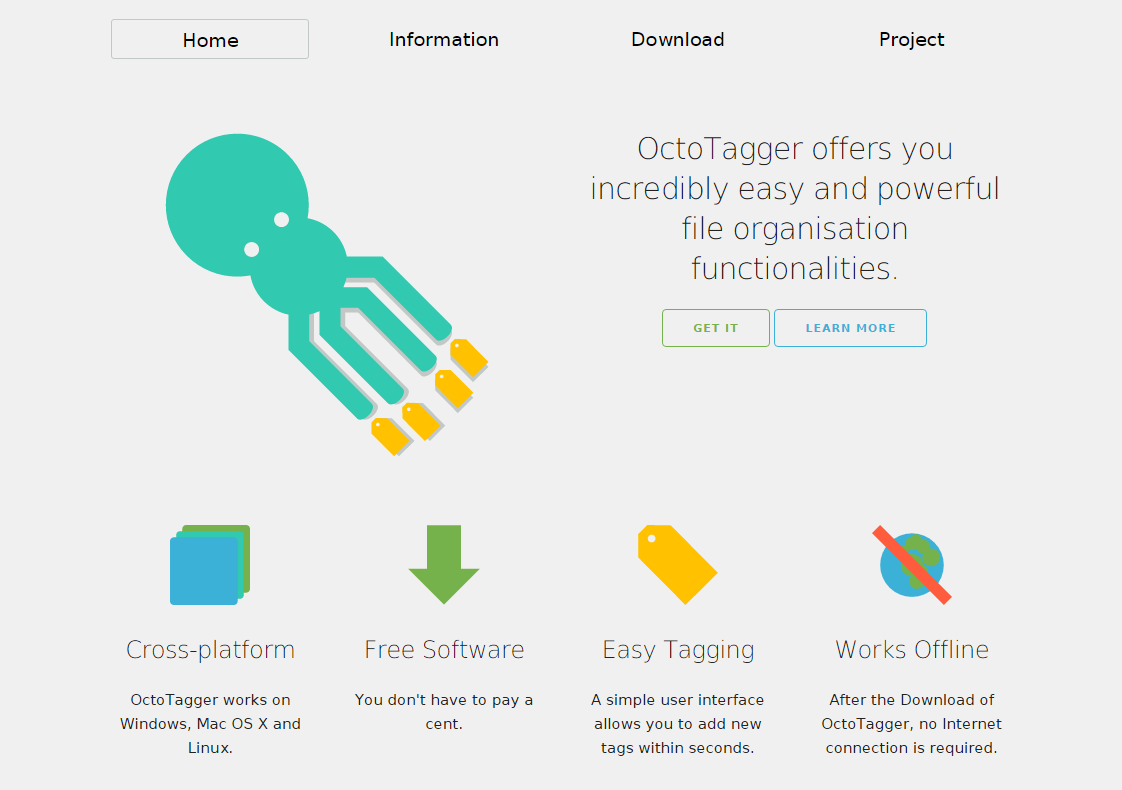
\includegraphics[scale=0.35]{images/home_full.png}\\
\end{center}

The home page is the first thing a user sees when he visits octotagger.co. This page is designed to catch the users attention with the help of a catchy slogan. The button "Learn more" is linked to the information page and with the help of the button "Get it" the user gets transferred to the download page. By just hovering the "Get it" button, a drop down menu appears and offers the possibility to directly download OctoTagger for the users operating system (see \ref{sec:OSdetection}). This option just makes sense, when the user has already installed the required software, of course.

In the bottom part the highlights of the software are pointed out with pictograms and short descriptions. The goal is to show the user the advantages of the software in one glance.

\subsubsection{Information page}

\begin{center}
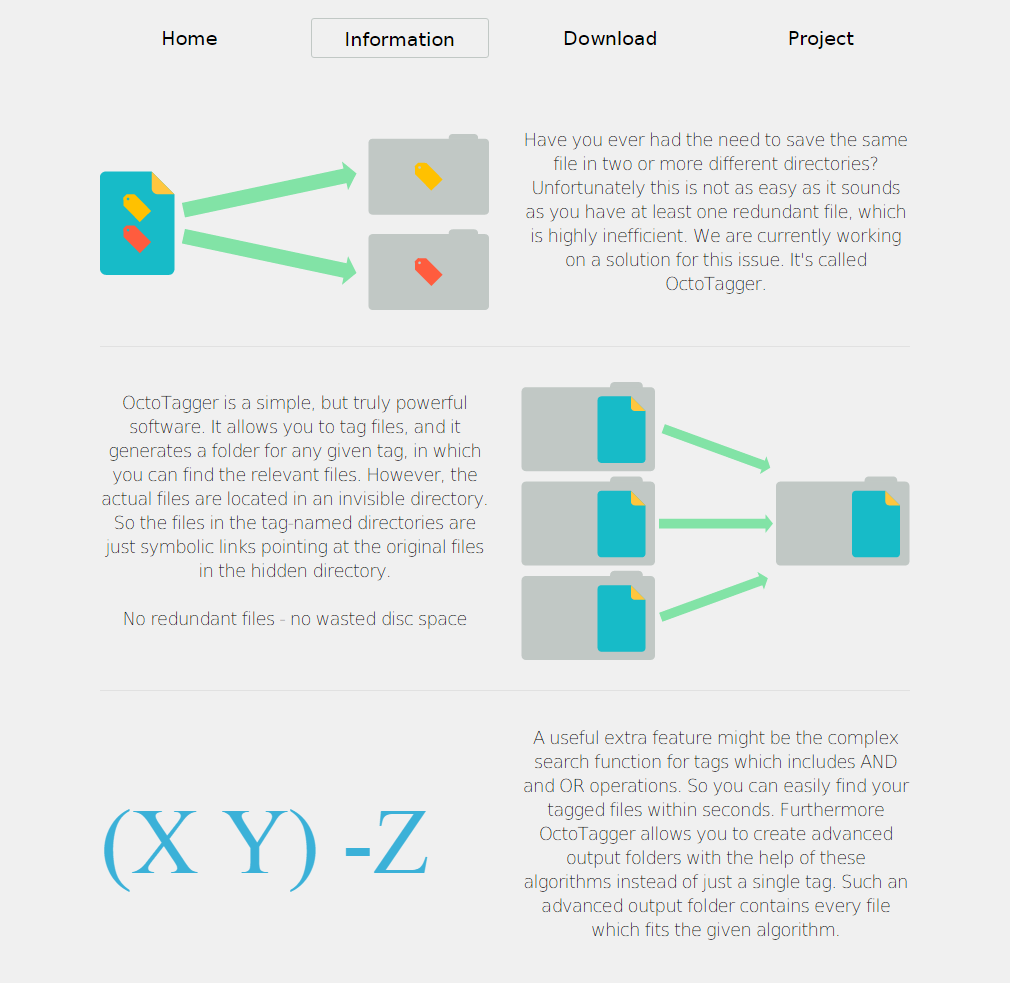
\includegraphics[scale=0.35]{images/information_full.png}
\end{center}

The information page offers the user some basic information about the functionality of OctoTagger. For this purpose, some simple images with short explanation text is shown. There is no previous knowledge needed to understand the explanation and the user doesn't have to deal with technical details.

\subsubsection{Download page}

\begin{center}
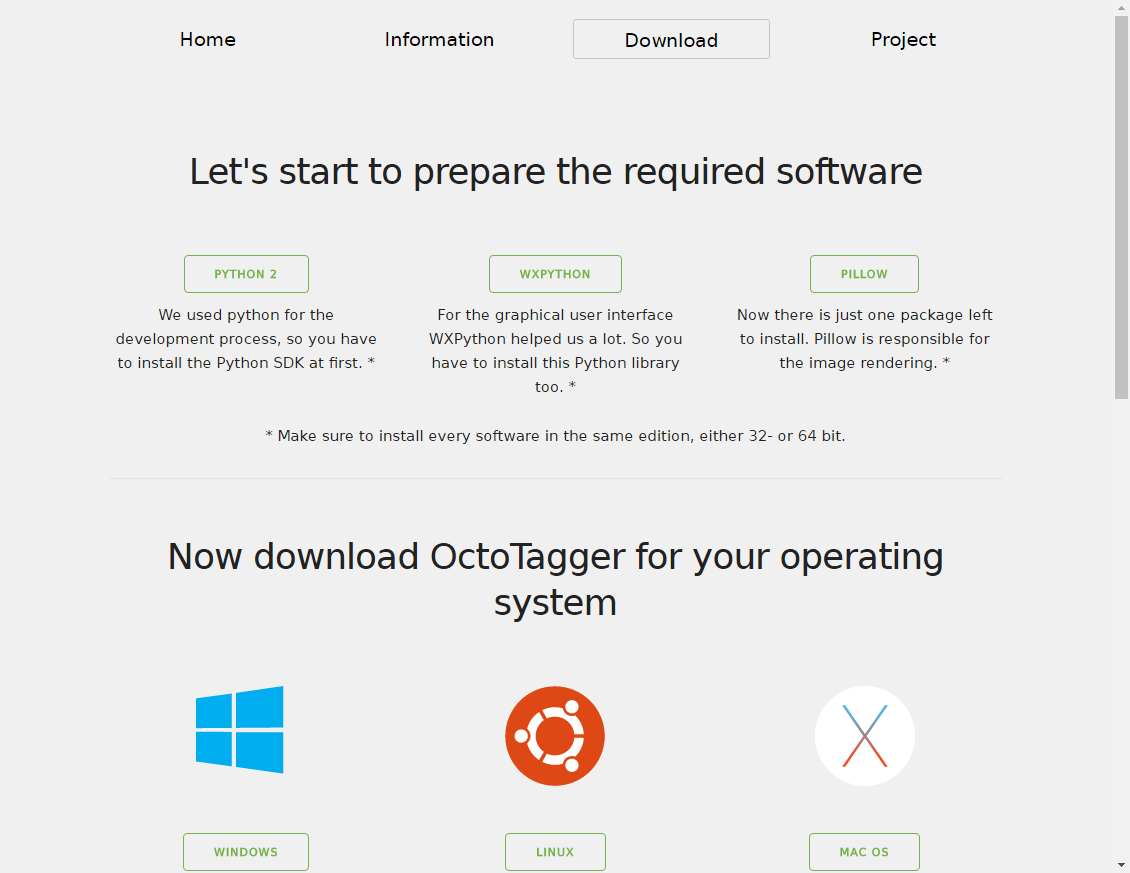
\includegraphics[scale=0.35]{images/download_full.png}
\end{center}

This page contains every available download and instructions for the installation. It's built like a step by step tutorial to guide the user through the entire process.

At first the user has to install the required software. The buttons on the top link to the developer website of the software. When a button is hovered, a dropdown menu shows up and offers the option to just show the installation instructions. When the button is clicked the download site as well as the instructions are opened in new tabs.
 
The second step describes the installation of OctoTagger itself. The download button provides the same functionality as the buttons above. By clicking this button the download starts directly and an installation guide opens in a new tab again. Windows user also have to install the OctoTagger Pywinlink service to be able to use OctoTagger afterwards.

In the last step the user has the possibility to download the user manual as PDF.

On the bottom of the page a link to our Git repository can also be found.

\subsubsection{Project page}

\begin{center}
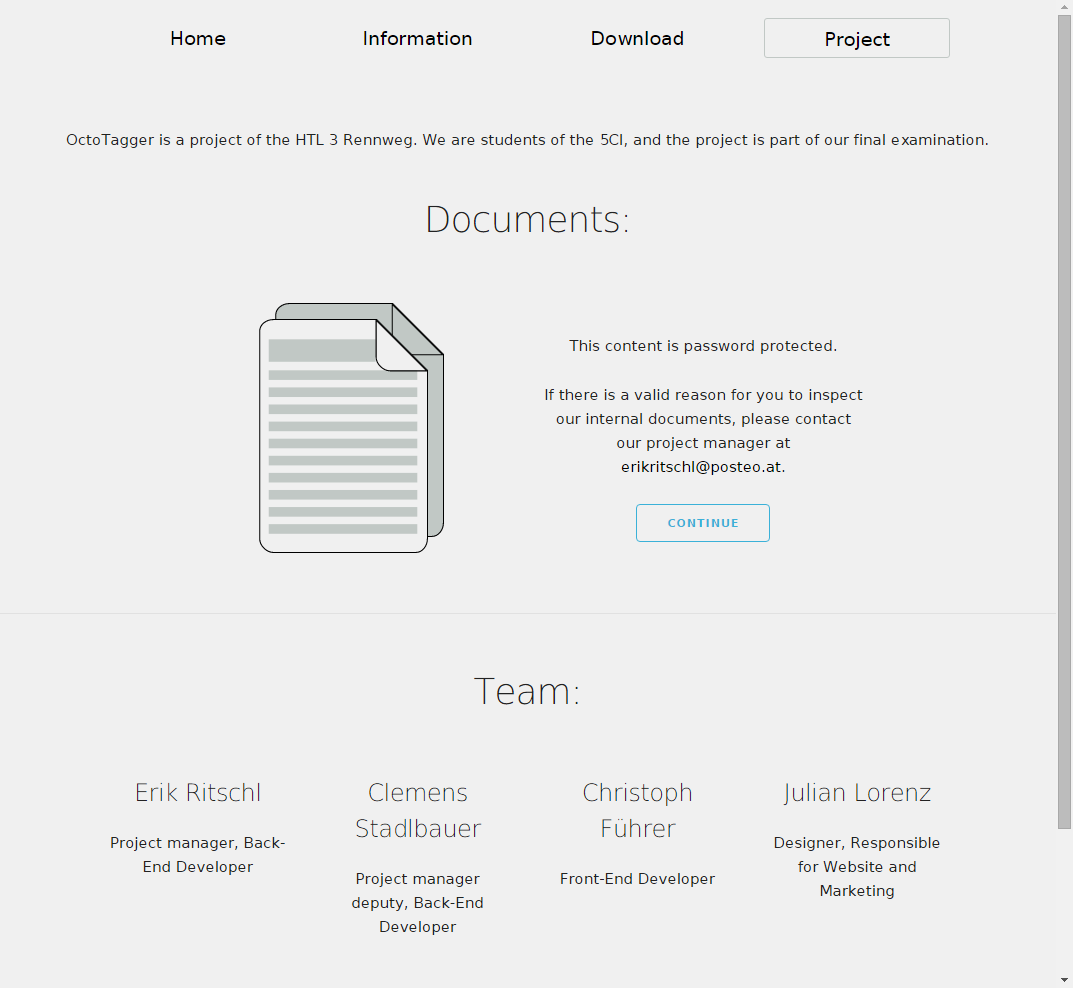
\includegraphics[scale=0.35]{images/project_full.png}
\end{center}

On this page information about the team, contact details and a link to some of our internal documents are brought together. 

\subsection{Used Tools and Technologies}

The following software, tools and frameworks helped us a lot at developing the website. Large and complex frameworks have completely been avoided to reduce loading times.


\subsubsection{Skeleton (Responsive CSS Framework)}
\label{sec:Skeleton}

Skeleton (http://getskeleton.com) is a framework which supports you with responsive development. Its source code consists of extremely few lines of code, making it great for small websites. Because of that Skeleton requires a lot of work of the developer and is basically only capable of managing the responsive grid system. It's everything you would need for responsive design, but nothing more.

\subsubsection{Adobe Illustrator}

This vector graphics editor was used for the creation of the images. 

\subsubsection{Sublime Text (Editor)}

\subsubsection{Operation System detection}
\label{sec:OSdetection}

Javascript allows the developer to check the user's operating system within just one line of code.



\subsection{Hosting}

The server is operated by the cloud provider Cloudatcost. This provider was chosen due to positive experiences in past projects and the possibility to buy a server for all time by a one-time payment. In addition, the price of 35 \$ for a simple web server is affordable for our project team. 

The server provides more then enough processing power for our needs and it's possible to install every available software on it thanks to command line control.

Namecheap was our choice concerning the purchase of the domain. This made another 8.88 \$ to use octotagger.co for one year.